%\documentclass{article}
%\usepackage{graphicx,subfigure}
%\begin{document}

\begin{figure}[!h]
  \centering
  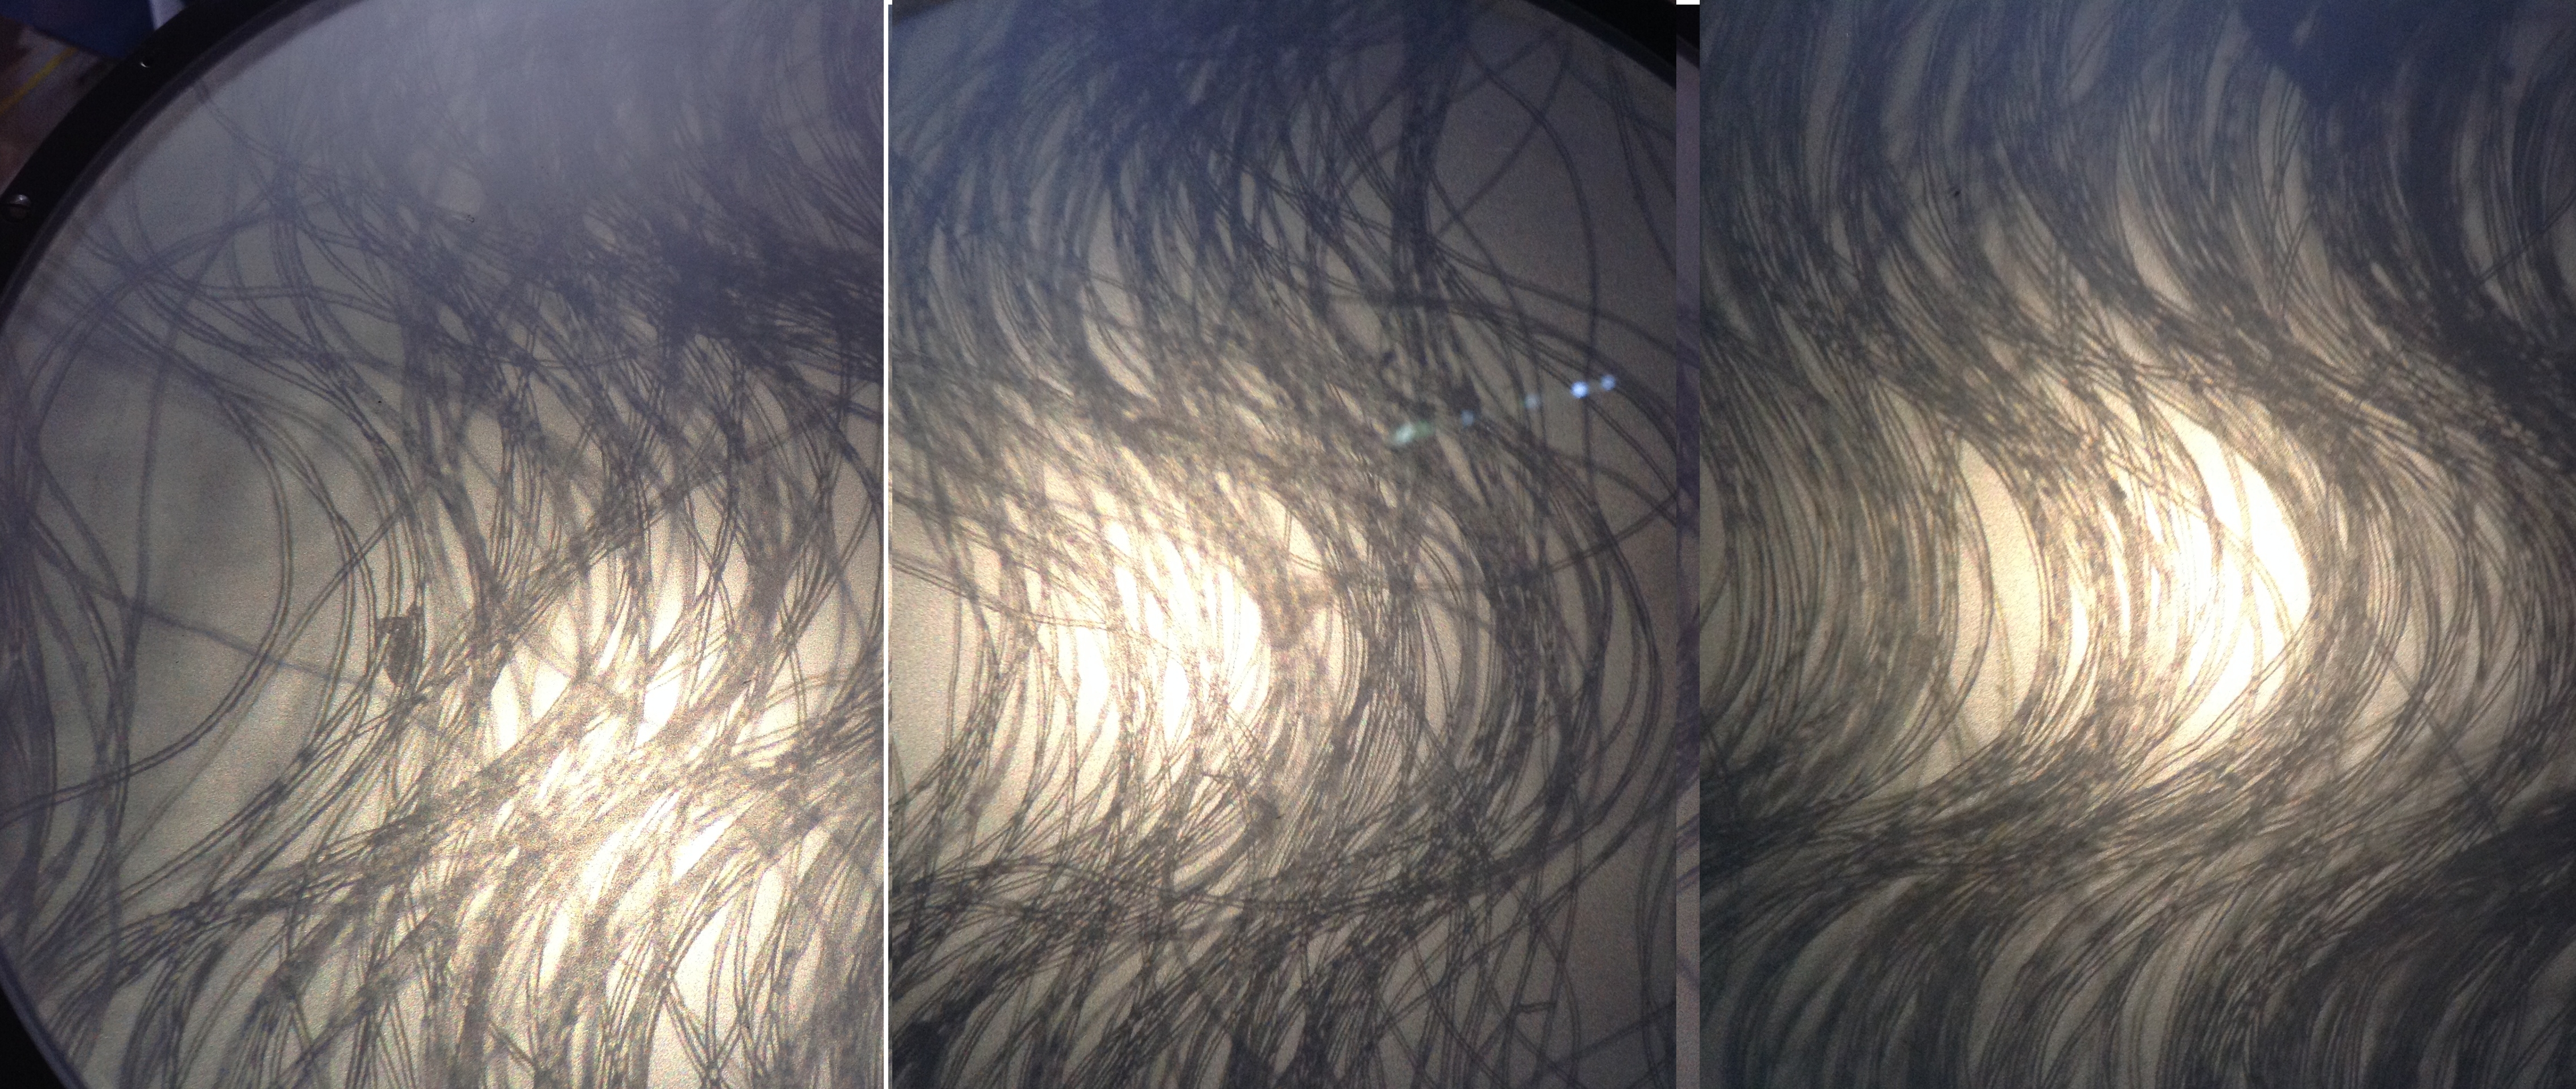
\includegraphics[width=1.0\textwidth]{figthreetypes.jpg}
%   composite of unalfib549.jpg, strebun574.jpg, unfobun.jpg
  \caption{Photomicrographs showing multiple bundles of fibres for each of the three staple crimp types shown in Figure~\ref{fig:woolphoto}. Left to right {\em unaligned}, {\em stretched}, and {\em unfolded}.  composite of unalfib549.jpg, strebun574.jpg, unfobun.jpg}
  \label{fig:threetypes}
\end{figure}

%\end{document}

